\documentclass[12pt]{article}
\setlength{\oddsidemargin}{0in}
\setlength{\evensidemargin}{0in}
\setlength{\textwidth}{6.5in}
\setlength{\parindent}{0in}
\setlength{\parskip}{\baselineskip}
\usepackage{amsmath,amsfonts,amssymb}
\usepackage{graphicx}
\usepackage{enumitem}
\usepackage[]{algorithmicx}
\usepackage{amsthm}
\usepackage{fancyhdr}
\pagestyle{fancy}
\setlength{\headsep}{36pt}

\usepackage{hyperref}

\theoremstyle{remark}
\newtheorem*{solution}{Solution}

\newcommand{\makenonemptybox}[2]{%
%\par\nobreak\vspace{\ht\strutbox}\noindent
\item[]
\fbox{% added -2\fboxrule to specified width to avoid overfull hboxes
% and removed the -2\fboxsep from height specification (image not updated)
% because in MWE 2cm is should be height of contents excluding sep and frame
\parbox[c][#1][t]{\dimexpr\linewidth-2\fboxsep-2\fboxrule}{
  \hrule width \hsize height 0pt
  #2
 }%
}%
\par\vspace{\ht\strutbox}
}
\makeatother

\begin{document}

\lhead{{\bf CSCI 3104, Algorithms \\ Problem Set 4a (11 points)} }
\rhead{Name: Luna McBride \\ ID: 107607144 \\ {\bf Profs.\ Hoenigman \& Agrawal\\ Fall 2019, CU-Boulder}}
\renewcommand{\headrulewidth}{0.5pt}

\phantom{Test}

\begin{small}
\textbf{Instructions for submitting your solution}:
\vspace{-5mm} 

\begin{itemize}
	\item The solutions \textbf{should be typed} and we cannot accept hand-written solutions. \href{http://ece.uprm.edu/~caceros/latex/introduction.pdf}{Here's a short intro to Latex.}
	\item You should submit your work through \href{https://www.gradescope.com/courses/59294}{\textbf{Gradescope}} only.
	\item If you don't have an account on it, sign up for one using your CU email. You should have gotten an email to sign up. If your name based CU email doesn't work, try the identikey@colorado.edu version. 
	\item Gradescope will only accept \textbf{.pdf} files (except for code files that should be submitted separately on Gradescope if a problem set has them) and \textbf{try to fit your work in the box provided}. 
	\item You cannot submit a pdf which has less pages than what we provided you as Gradescope won't allow it. 
	\item Verbal reasoning is typically insufficient for full credit. Instead, write a logical argument, in the style of a mathematical proof.
	\item For every problem in this class, you must justify your answer:\ show how you arrived at it and why it is correct. If there are assumptions you need to make along the way, state those clearly.
	
	\item You may work with other students. However, \textbf{all solutions must be written independently and in your own words.} Referencing solutions of any sort is strictly prohibited. You must explicitly cite any sources, as well as any collaborators. 
\end{itemize}
\vspace{-4mm} 
\end{small}

\hrulefill

\newpage
\begin{enumerate}
\item (1 pt) What is the definition of a Minimum Spanning Tree (MST)?
\begin{solution}
$\newline$ A Spanning Tree is a graph who has as few connections as possible to make sure every vertex connected to at least one other vertex. These can be obtained from removing edges from a regular graph such that there is only those edges necessary to connect all vertices. $\newline$ As an extension, the Minimum Spanning Tree is a Spanning Tree that removes the edges to the connections have the smallest weight possible.
\end{solution}
\item (1 pt) Describe in one or two sentences, a greedy rule for constructing an MST.
\begin{solution}
$\newline$ The Kruskals method takes the set of edges in a graph, organizes it by minimum size, then goes one by one with the minimums, checking if it creates a loop with others already in the solution set. If not, said value is added to the solution set, which is used to show which edges would be used in a MST.
\end{solution}

\item (3 pts) How many unique MSTs does the following graph have :
\begin{figure}[h!]
\begin{center}
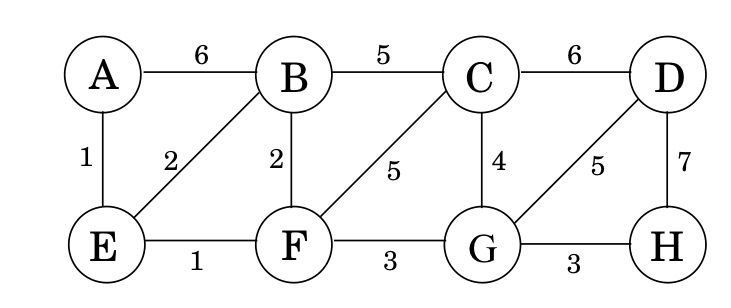
\includegraphics[scale=0.3]{mst_graph_q2.jpg} 
\end{center}
\end{figure}


\begin{solution}
$\newline 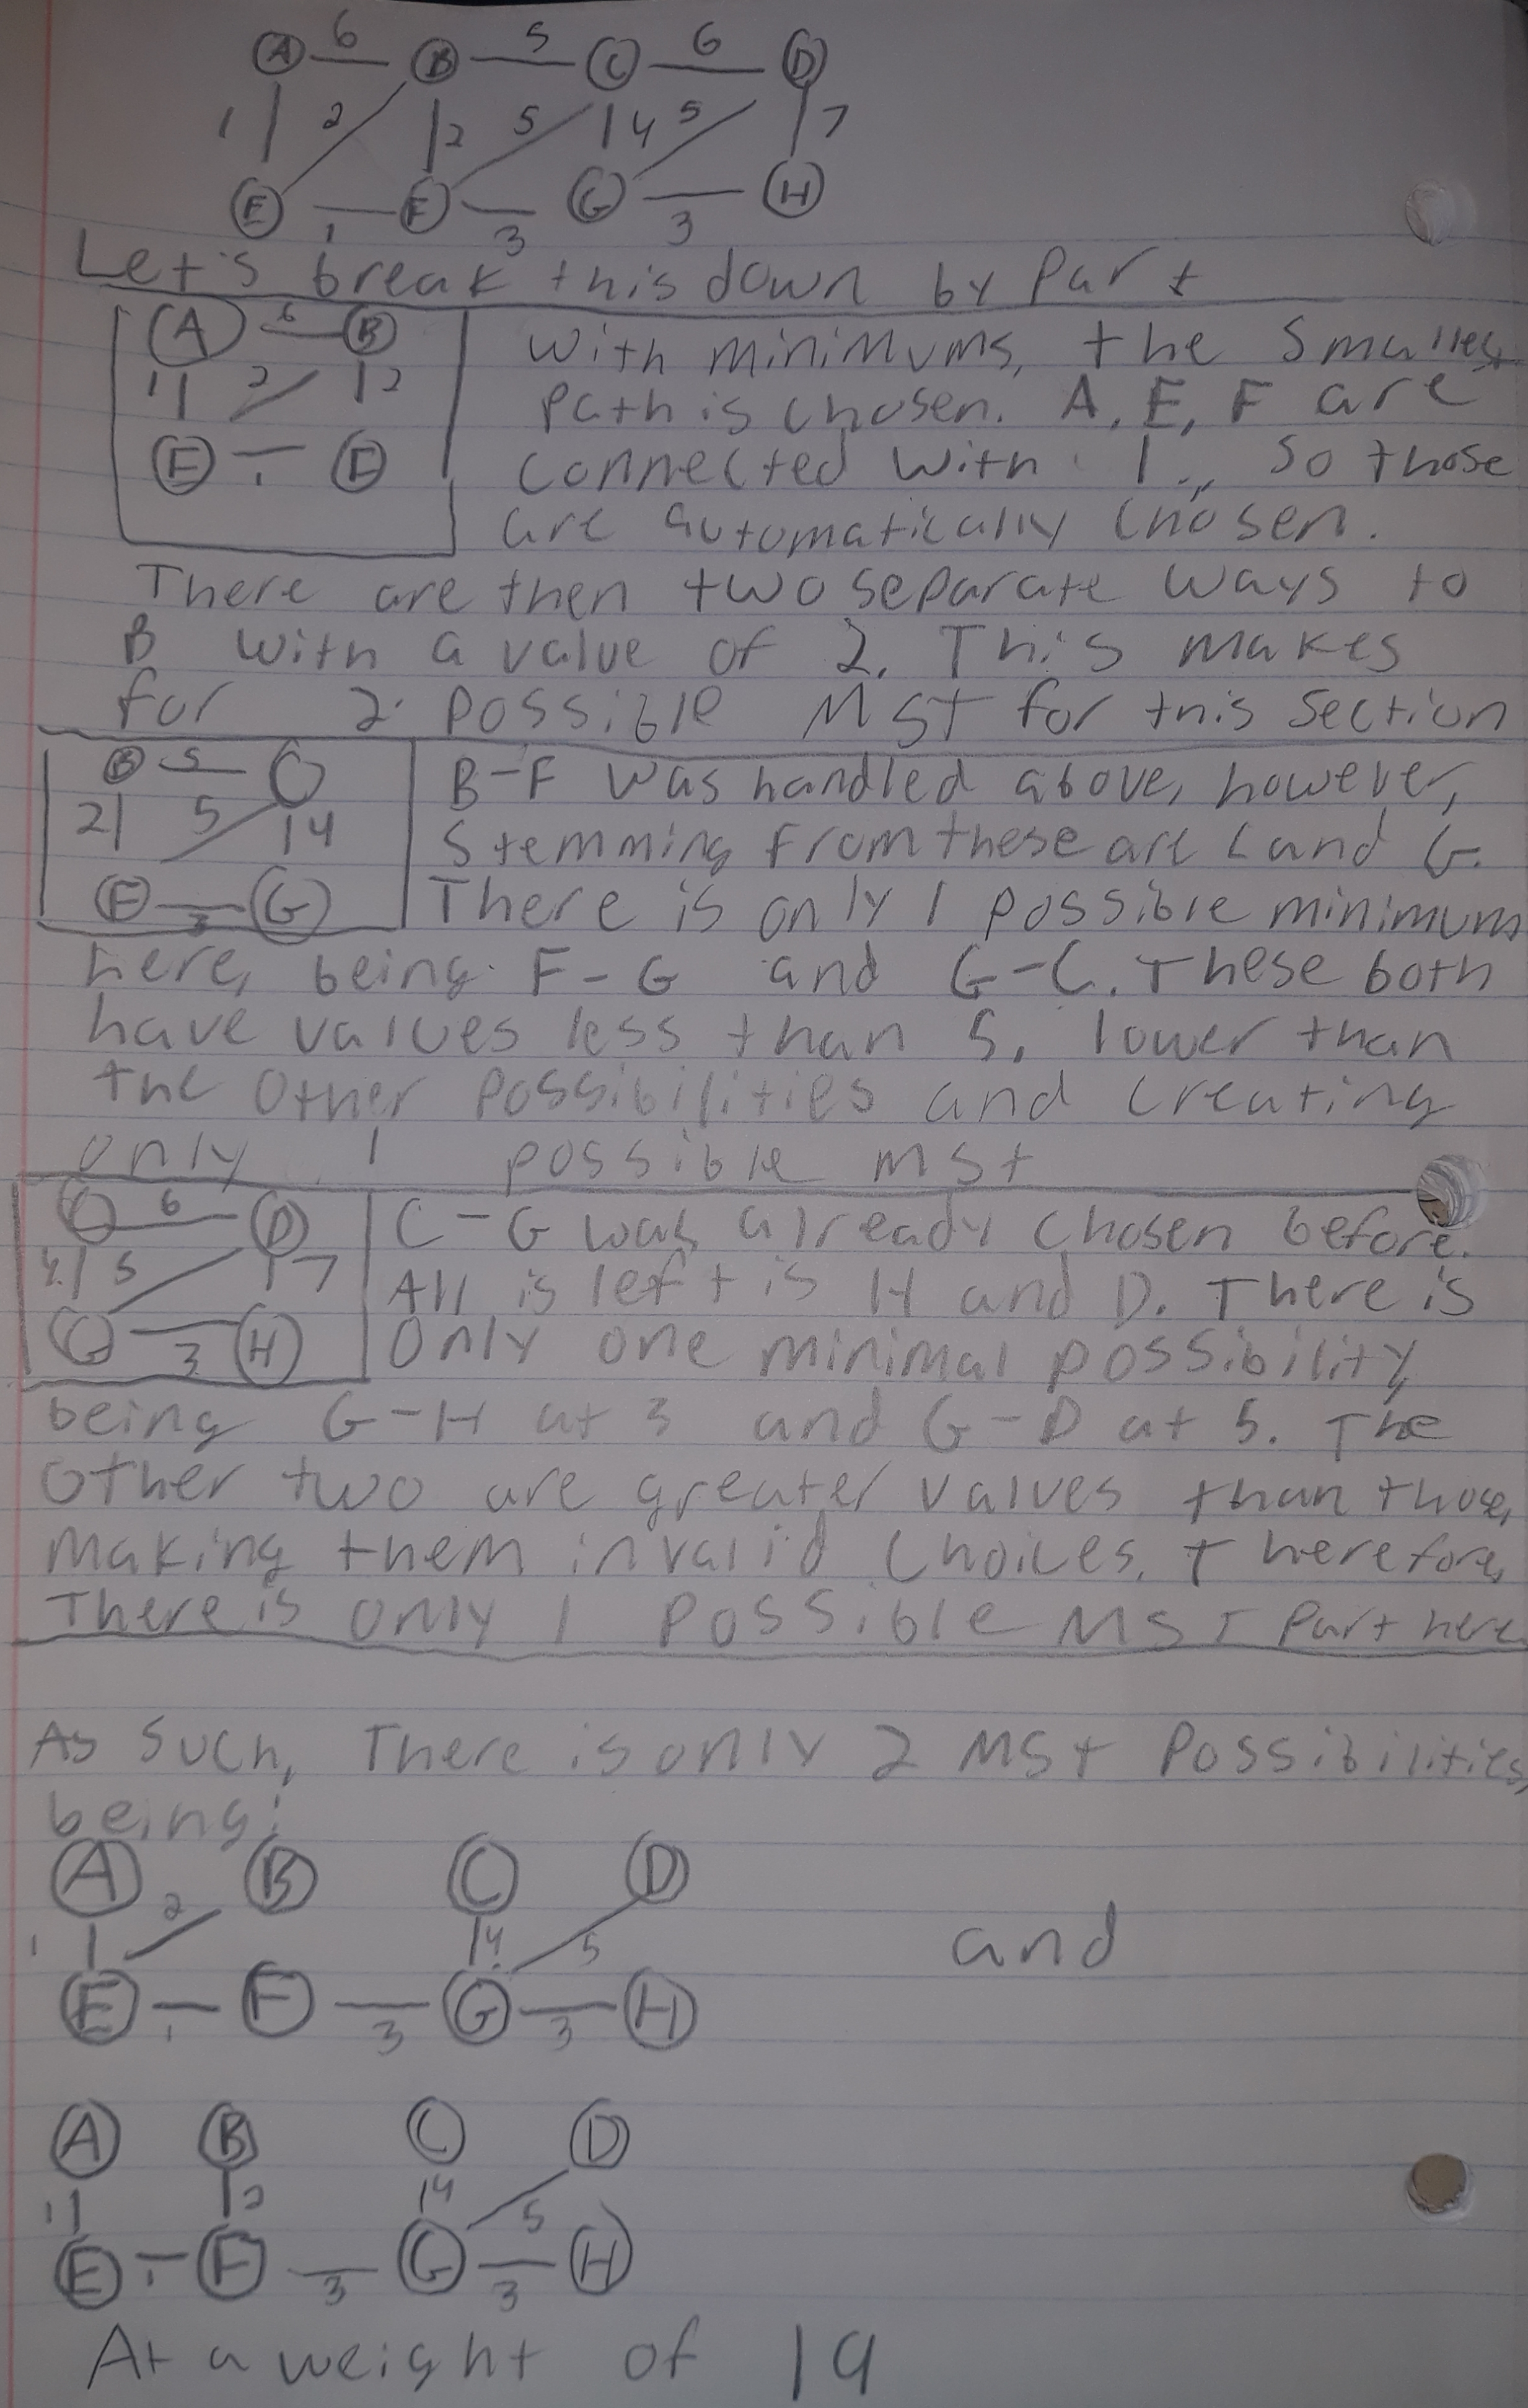
\includegraphics[width=\textwidth, height=7.75in]{MST} $
\end{solution}

\pagebreak
\item (3 pts) Suppose that you have calculated the MST of an undirected graph $G=(V,E)$ with positive edge weights. \\
If you increase each edge weight by 2, will the MST change? Prove that it cannot change or give a counterexample if it changes. (Note: Your proof, if there is one, can be a simple logical argument.)
\begin{solution}
$\newline$ For this, let us take the graph from the previous question and add 2 to each value: $\newline$ 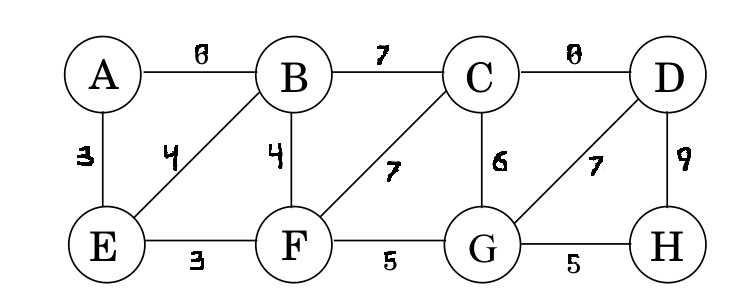
\includegraphics[scale=1]{mst_graph_q2-2} $\newline \newline$ As can be seen, each value is still the same in proportion to one another. The MST will still have the same structure, as the value that is lowest is still the lowest. Going through the same math hoops as before, on this graph, I got this MST, where the dashed lines represent the two that could be picked for different unique trees: 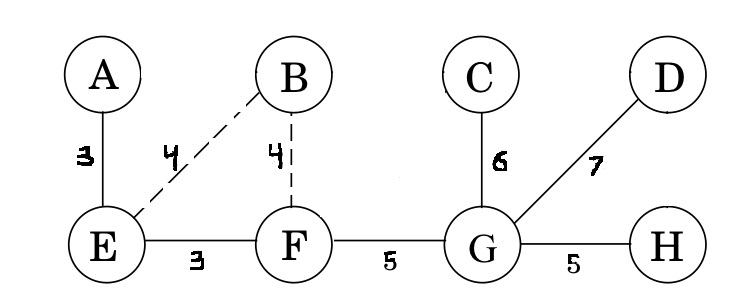
\includegraphics[scale=1]{mst_graph_q2-3} $\newline$ This is the same shape as above. This shows that adding 2 to everything will not change anything.

\end{solution}
\pagebreak

\item (3 pts) Suppose that you have calculated the shortest paths to all vertices from a fixed vertex $s\in V$ of an undirected graph $G=(V,E)$ with positive edge weights. \\
If you increase each edge weight by 2, will the shortest paths from $s$ change? Prove that it cannot change or give a counterexample if it changes.(Note: Just as in Part a, your proof can be a simple logical argument.)
\begin{solution}
$\newline$ As stated above, adding 2 for everything proportionally increases values, leaving the smallest as the smallest. This means the shortest is still relatively the shortest, and thus the shortest path. $\newline \newline$ Base case: A$-->$B=2 changes to A$-->$B=4, which is still the shortest between the only two points. $\newline \newline$ Inductive Hypothesis: Say for path of length k, the path is still the same with each weight being added by 2. $\newline \newline$ Inductive Step: $\newline \newline$ ----Case 1: There is only one way to possibly go besides to next node v. No matter the addition of 2, the next way is the next way and must be taken. $\newline$ ----Case 2: There are multiple applicable paths. In this, we have to follow the proportion of those branches, look for the smallest, then continue. If we add 2 to each of those values, they are the same proportion to one another. For example, we could have weights 3 and 6. Those become 5 and 8, which still makes them different by 3. The 3 path (now the 5 path) will still be chosen by still being the smallest proportionally and the 6 path (now the 8 path) will still be neglected at the current moment. $\newline \newline$ Therefore, we can reasonably say the paths will remain the same despite every value being increased by 2.
\end{solution}

\pagebreak


\end{enumerate}

\end{document}


